\documentclass[a4paper]{article}
\usepackage[margin=2cm]{geometry}
\usepackage{fancyhdr}
\pagestyle{fancy}
\fancyhead[CO,CE]{
                  Programming in C/C++ \\
                  Tjalling Otter \& Emiel Krol
                 }

\usepackage{etoolbox}
\usepackage{placeins}
\usepackage{float}
\usepackage{graphicx}

\usepackage[usenames,dvipsnames]{color}  %% Allow color names

% New page for every section
\let\stdsection\section
\renewcommand\section{\newpage\stdsection}

% New page for every subsection
%\let\stdsubsection\subsection
%\renewcommand\subsection{\newpage\stdsubsection}

%% The listings package will format your source code
\usepackage{listings}
\lstdefinestyle{customasm}{
  title=\lstname,
  belowcaptionskip=1\baselineskip,
  language=C++,
  breaklines=true, %% Wrap long lines
  basicstyle=\small\ttfamily,
  commentstyle=\color{Gray},
  stringstyle=\color{Black},
  keywordstyle=\bfseries\color{OliveGreen},
  identifierstyle=\color{blue},
  numbers=left,
  showstringspaces=false
}

\lstdefinestyle{text}{
  title=\lstname,
  belowcaptionskip=1\baselineskip,
  breaklines=true, %% Wrap long lines
  basicstyle=\small\ttfamily,
  showstringspaces=false,
  breakautoindent=true
}

%\newtoggle{aftersection}
%\preto{\lstinputlisting}{\filbreak\global\toggletrue{aftersection}}
%\preto{\subsection}{\iftoggle{aftersection}{\global\togglefalse{aftersection}}{\filbreak}}
%\newcommand{\clearpageafterfirst}{%
%  \gdef\clearpageafterfirst{\clearpage}%
%}

\begin{document}

\section*{Week 5}

\subsection*{Exercise 40}
\lstinputlisting[style=text]{../40/40.txt}
\begin{figure}[H]
\centerline{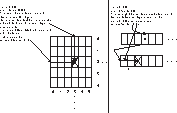
\includegraphics[trim={0 0cm 0 0cm}, scale=5]{../40/illustration.pdf}}
\caption{Illustration}
\end{figure}

%\newpage
\subsection*{Exercise 41}
\lstinputlisting[style=customasm]{../42-2/main.ih}
\lstinputlisting[style=customasm]{../42-2/main.cc}
\lstinputlisting[style=customasm]{../42-2/showChar.cc}
\lstinputlisting[style=customasm]{../42-2/charcount/charcount.ih}
\lstinputlisting[style=customasm]{../42-2/charcount/charcount.h}
\lstinputlisting[style=customasm]{../42-2/charcount/charsorter.cc}
\lstinputlisting[style=customasm]{../42-2/charcount/constructor.cc}
\lstinputlisting[style=customasm]{../42-2/charcount/enlarge.cc}
\lstinputlisting[style=customasm]{../42-2/charcount/existsCheck.cc}
\lstinputlisting[style=customasm]{../42-2/charcount/firstChar.cc}
\lstinputlisting[style=customasm]{../42-2/charcount/info.cc}
\lstinputlisting[style=customasm]{../42-2/charcount/newChar.cc}
\end{document}
